% Relatório do laboratório 3 de servo
% Felipe Bandeira da Silva
% 09/06/2013

\documentclass[a4paper, 10pt]{article}

\usepackage[brazil]{babel}
\usepackage[utf8]{inputenc}

\usepackage{listings}
\usepackage{color}

\usepackage{amsthm}


%\usepackage[pdftex]{graphicx}
%\graphicspath{{../pdf/}{../jpeg/}}
\usepackage{graphicx}


\title{Relatório do Laboratório 3}
\author{Felipe Bandeira da Silva}
\begin{document}
\maketitle


%\tableofcontents


%\lstset{language = Matlab}

% http://en.wikibooks.org/wiki/LaTeX/Source_Code_Listings

\definecolor{mygreen}{rgb}{0,0.6,0}
\definecolor{mygray}{rgb}{0.5,0.5,0.5}
\definecolor{mymauve}{rgb}{0.58,0,0.82}

\lstset{ %
  backgroundcolor=\color{white},   % choose the background color; you must add \usepackage{color} or \usepackage{xcolor}
  basicstyle=\footnotesize,        % the size of the fonts that are used for the code
  breakatwhitespace=false,         % sets if automatic breaks should only happen at whitespace
  breaklines=true,                 % sets automatic line breaking
  captionpos=b,                    % sets the caption-position to bottom
  commentstyle=\color{mygreen},    % comment style
  deletekeywords={...},            % if you want to delete keywords from the given language
  escapeinside={\%*}{*)},          % if you want to add LaTeX within your code
  extendedchars=true,              % lets you use non-ASCII characters; for 8-bits encodings only, does not work with UTF-8
  frame=single,                    % adds a frame around the code
  keepspaces=true,                 % keeps spaces in text, useful for keeping indentation of code (possibly needs columns=flexible)
  keywordstyle=\color{blue},       % keyword style
  language=Matlab,                 % the language of the code
  morekeywords={*,...},            % if you want to add more keywords to the set
  numbers=left,                    % where to put the line-numbers; possible values are (none, left, right)
  numbersep=5pt,                   % how far the line-numbers are from the code
  numberstyle=\tiny\color{mygray}, % the style that is used for the line-numbers
  rulecolor=\color{black},         % if not set, the frame-color may be changed on line-breaks within not-black text (e.g. comments (green here))
  showspaces=false,                % show spaces everywhere adding particular underscores; it overrides 'showstringspaces'
  showstringspaces=false,          % underline spaces within strings only
  showtabs=false,                  % show tabs within strings adding particular underscores
  stepnumber=2,                    % the step between two line-numbers. If it's 1, each line will be numbered
  stringstyle=\color{mymauve},     % string literal style
  tabsize=2,                       % sets default tabsize to 2 spaces
  title=\lstname                   % show the filename of files included with \lstinputlisting; also try caption instead of title
}






%\section{Expansão em frações parciais}
 \newcounter{quest}
\begin{list}{\textbf{Questão \arabic{quest}.}}{\usecounter{quest}
\setlength{\labelwidth}{-2mm} \setlength{\parsep}{0mm}
\setlength{\topsep}{0mm} \setlength{\leftmargin}{0mm}}
\renewcommand{\labelenumi}{(\alph{enumi})}

\item Faça a expansão em frações parciais das funções abaixo com o auxílio do Matlab
e em seguida obtenha a transformada inversa de laplace.
    \begin{enumerate}
        \item       
            $$ 
                F(s) = \frac{10(s+2)(s+4}{(s+1)(s+3)(s+5)^2}
            $$

Usando a seguinte sequência de comandos para a obtenção da expansão,
            \begin{lstlisting}
a = [1 2];
b = [1 4];
num = 10*conv(a, b);
a = [1 1];
b = [1 3];
c = [1 5];
den = conv(conv(a, b), conv(c, c));
[r, p, k] = residue(num, den);

            \end{lstlisting}


        Resultado,

        \begin{lstlisting}
r = 
   -2.1875 
    3.7500
    1.2500
    0.9375

p = 
   -5.0000
   -5.0000
   -3.0000
   -1.0000

k = 
   []

        \end{lstlisting}
        Rearranjando os valores do resíduos, polos e termo de evidenciamento,

            $$
                F(s) = \frac{-2.1875}{s+5} + \frac{3.75}{s+5} + \frac{1.25}{s+3} + \frac{0.9375}{s+1}
            $$

            Aplicando a transformada inversa de laplace,

            $$
            f(t) = -2.1875 e^{-5t} + 3.75 e^{-5t} + 1.25 e^{-3t} + 0.9375 e^{-t}
            $$
         


    \item

        $$
        F(s) = \frac{s+1}{s(s^2+s+1)}
        $$

        Usando a mesma ideia usando no item (a) é possível obter, 

        \begin{lstlisting}
r = []
p = []
k = []
    \end{lstlisting}


    \item

        $$
        F(s) = \frac{2 s^3 + 5 s^2 + 3 s + 6}{s^3 + 6 s^2 + 11 s + 6}
        $$

        Usando a mesma ideia usando no item (a) é possível obter, 

        \begin{lstlisting}
r = 
   -6.0000
   -4.0000
    3.0000
p = 
   -3.0000
   -2.0000
   -1.0000
k = 
    2
    \end{lstlisting}


        Rearranjando os termos, 

        $$
        F(s) = \frac{-6}{s+3} + \frac{-4}{s+2} + \frac{3}{s+1} + 2
        $$

        Aplicando a transformada inversa de laplace,

        $$
        f(t) = -6 e^{-3t} -4 e^{-2t} + 3 e^{-t} + 2 \delta(t)
        $$

    \end{enumerate}











\item 
    Com base no sistema definido pela seguinte função de transferência, obtenha:

    $$
    G(s) = \frac{Y(s)}{X(s)} = \frac{3}{s(s+1)}
    $$
    \begin{enumerate}
        \item
            Função temporal $y(t)$ que representa a resposta do sistema quando excitado
            por um impulso unitário $x(t)=\delta(t)$ e rampa unitário $x(t)=r(t)$ \\

            O $\mathcal{L}(\delta(t)) = 1$ com isto é possível obter a resposta 
            $Y(s)$ ao impulso, 
    
            $$
                Y(s) = \frac{3}{s(s+1)} \cdot 1
            $$

            Usando o comando "residue" para a expansão em frações parciais, temos,

            $$
                Y(s) = -\frac{3}{s+1} + \frac{3}{s}
            $$

            Aplicando $\mathcal{L}^{-1}$,

            $$
            \mathcal{L}^{-1}Y(s)=\mathcal{L}^{-1}( -\frac{3}{s+1} + \frac{3}{s} ),
            $$

            Resolvendo para $t$,

            $$
                y(t) = 3 - 3 e^{-t}
            $$\\

            

            Para o degrau unitário o $\mathcal{L}(u(t)) = \frac{1}{s}$, a resposta a excitação,

            $$
            Y(s) = \frac{3}{s(s+1)} \cdot \frac{1}{s} = \frac{3}{s^3+s^2}
            $$

            Expandindo em frações parciais,

            $$
            Y(s) = \frac{3}{s+1} - \frac{3}{s} + \frac{3}{s^2} 
            $$

            Aplicando $\mathcal{L}^{-1}$,

            $$
            y(t) = 3 - 3 t + 3 e^{-t}
            $$\\


            Para a ultima resposta, a $\mathcal{L}$ da rampa unitária é $\mathcal{L}(r(t)) = \frac{1}{s^2}$, logo,

            $$
            Y(s) = \frac{3}{s(s+1)} \cdot \frac{1}{s^2} = \frac{3}{s^4 + s^3}
            $$

            Expandindo em frações parciais,

            $$
            Y(s) = \frac{3}{s^3} - \frac{3}{s^2} + \frac{3}{s} - \frac{3}{s+1}
            $$

            Aplicando $\mathcal{L}^{-1}$,


            $$
            y(t) = \frac{3 t^2}{2} - 3 t + 3 - 3 e^{-t}
            $$

            \newpage
         \item 
             Apresente um um mesmo gráfico a resposta $y(t)$  obtida no item anterior, 
             considerando um intervalo de tempo de 0seg a 10seg com passo de 0.01seg.
 
             \begin{center}
                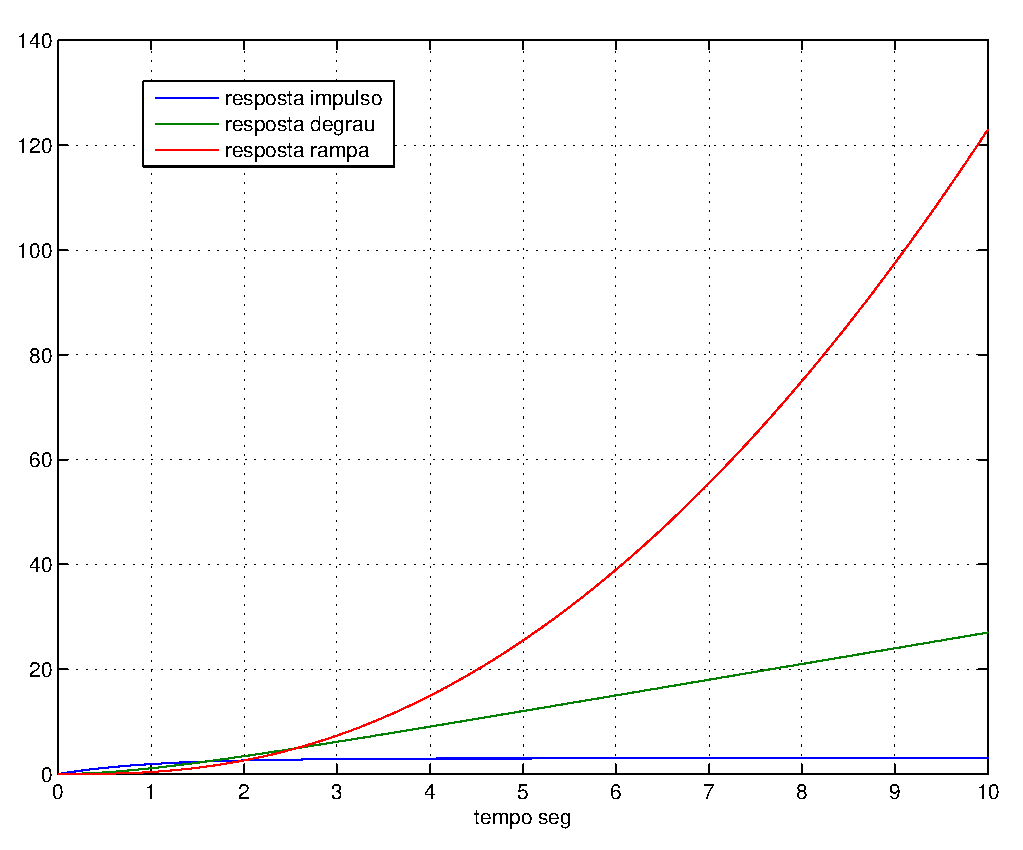
\includegraphics[scale=0.6]{fig2q.eps}
             \end{center}

             %\begin{figure}
             %   \centerline{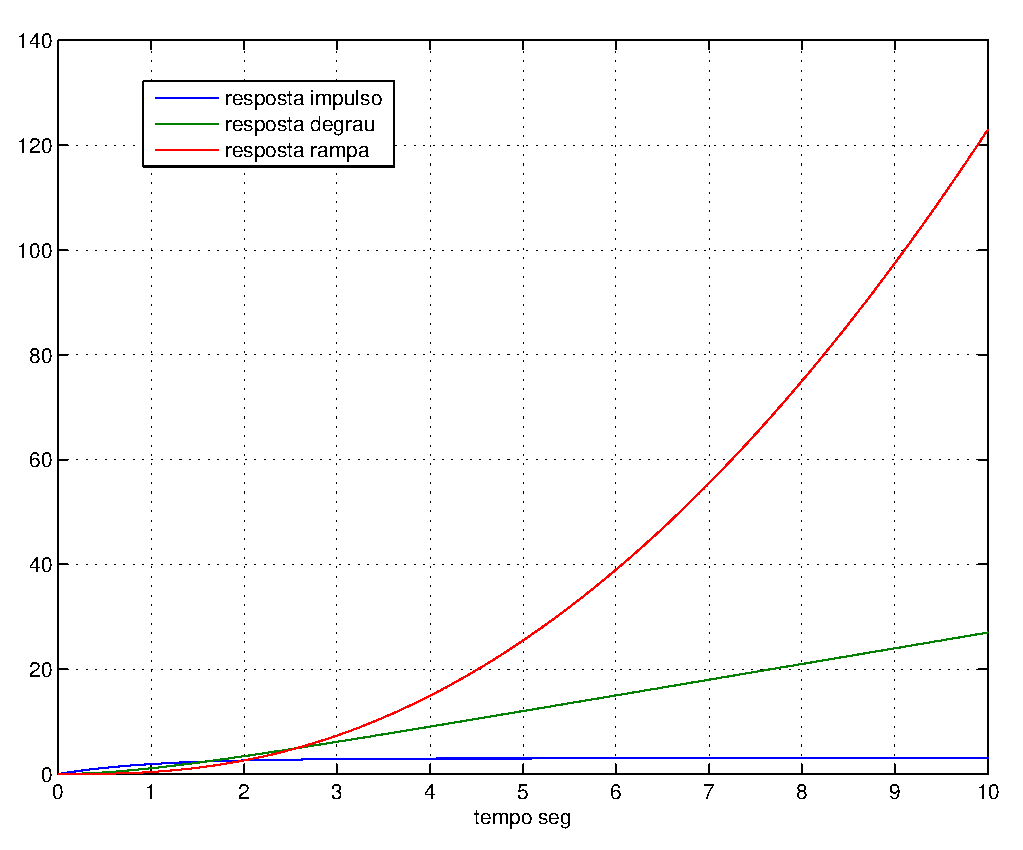
\includegraphics[scale=0.6]{fig2q.eps}
             %   \label{fig:TheFig}
             %   \caption{fefe}
             %\end{figure}

    \end{enumerate}

\newpage

\item
    Encontre os zeros, polos e ganho da função de transferência abaixo. Em seguida, 
    represente e identifique os polos e zeros no plano-s.

    $$
    G(s) = \frac{4 s^2 + 16 s + 12}{s^4 + 12 s^3 +  44 s^2 + 48 s}
    $$


    Para a solução deste problema, criei o seguinte código,

 
     \begin{lstlisting}
num = [4 16 12];
den = [1 12 44 48 0];
z = roots(num);
p = roots(den);
k = 1;
fun = zpk(z, p, k);
     \end{lstlisting}

     Obtendo os pólos e zeros no plano-s,
        \begin{center}
                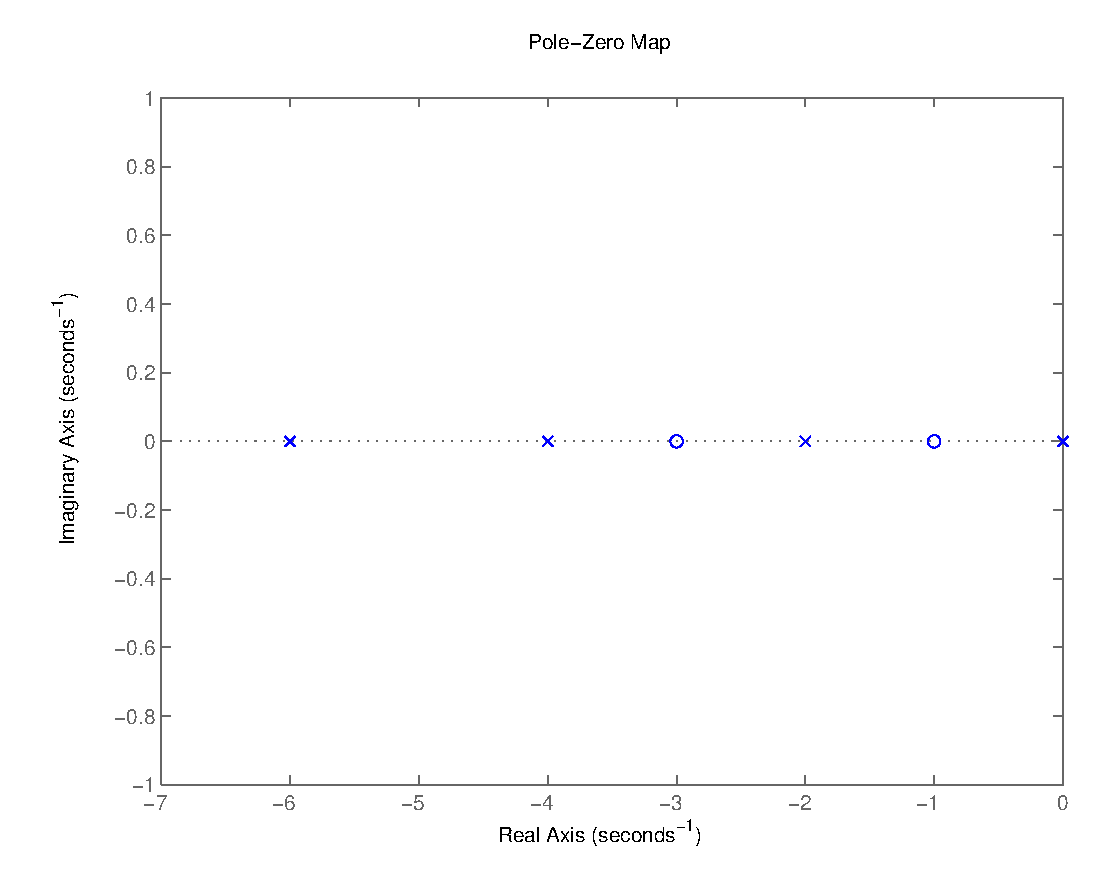
\includegraphics[scale=0.6]{fig3q.eps}
             \end{center}

     



\newpage

         \item
             Dados os zeros, pólos e ganho K a seguir, obtenha a função de transferência 
             que representa o respectivo sistema:
        \begin{enumerate}
            \item

                Não existe zeros, os pólos estão em $-2\pm5j$ e o ganho é 10.\\
                
                Para a solução, o seguinte código foi utilizado,

                \begin{lstlisting}
z = [];
p = [-2+5j -2-5j];
k = 10;
zpk(z, p, k);               
                \end{lstlisting}

                Resultando na seguinte função de trasnferência,

                $$
                G(s) = \frac{10}{s^2 + 4 s + 29}
                $$



             \item
                 O zero está em 0, os pólos estão em $-1\pm2j$ e o ganho é 1.\\

                 Usando o mesmo código usando no item a, a função de transferência fica,

                 $$
                 G(s) = \frac{s}{s^2 + 2 s + 5}
                 $$

                 

             \item
                 Os zeros estão em 0 e -1, os pólos estão em -2, -3 e 
                 $-2\pm5j$ e o ganho é 4.\\

                 A função de transferência é,

                 $$
                 G(s) = \frac{4 s (s+1)}{(s+2) (s+3) (s^2 + 4 s + 29)}
                 $$
                

        \end{enumerate}


\newpage
\item
    Obtenha a função de transferência equivalente dos sistemas abaixo, sendo:

    \begin{enumerate}
        \item
            Figura 1
            \begin{center}
            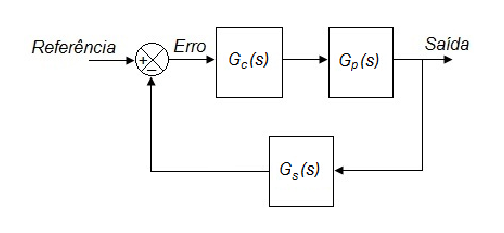
\includegraphics[scale=0.5]{fig5a.png}
            \end{center}

            Usando os comandos $series$ e $feedback$ é possivel criar a função
            de transferência, para tanto o codigo abaixo foi construido,

            \begin{lstlisting}
gc = tf([1 0],[1 1])
gp = tf([2], [1 1 2])
gs = tf([1], [1 0.5])
s = series(gc, gp)
f = feedback(s, gs)
             \end{lstlisting}

            Resultando na seguinte equação de transferência,

            $$
            H(s) = \frac{2 s^2 + s}{s^4 + 2.5 s^3 + 4 s^2 + 5.5 s + 1}
            $$


        \item
             Figura 2
            \begin{center}
            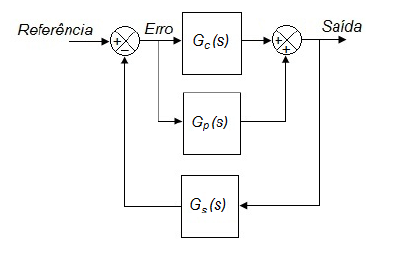
\includegraphics[scale=0.5]{fig5b.png}
            \end{center}
            
            Com uma pequena alteração do código usando no item a, para suportar
            a associação em paralelo

             \begin{lstlisting}
gc = tf([1 0],[1 1])
gp = tf([2], [1 1 2])
gs = tf([1], [1 0.5])
p = parallel(gc, gp)
f1 = feedback(p, gs)
             \end{lstlisting}

             Resultando na seguinte equação de transferência,

             $$
                H(s) = \frac{s^4 + 1.5 s^3 + 4.5 s^2 + 4 s + 1}{s^4 + 3.5 s^3 + 5 s^2 + 7.5 s + 3}
             $$


    \end{enumerate}


\newpage
\item
  Com base no sistema dinâmico abaixo, obtenha analiticamente as matrizes de estado
  \textbf{(A, B, C, D)} considerando o posição $x(t)$ e a velocidade $\frac{d x(t)}{dt}$
  com variáveis de estado, $F(t)$ como entrada e $x(t)$ como saída. Em seguida utilize
  o Matla para encontrar a função de transferência correspondente. Considere
  $m=1.0 kg$, $b=0.2 N s/m$, $k=3.0 N/m$

            \begin{center}
            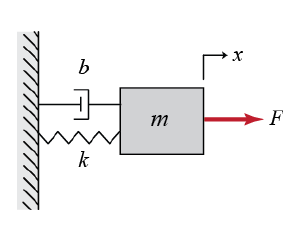
\includegraphics[scale=0.6]{fig6a.png}
            \end{center}
 
\newpage
\item
    Com o auxilio do Matlab, obtenha as matrizes de estado $\textbf(A, B, C, D)$ do 
    sistema mostrado a seguir:
            \begin{center}
            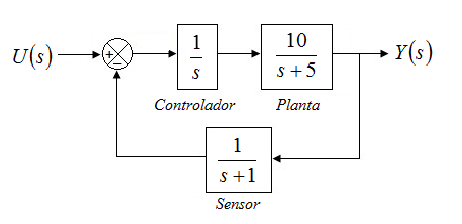
\includegraphics[scale=0.6]{fig7.png}
            \end{center}
 
\end{list}


\end{document}

